\documentclass[12pt]{article}

\usepackage[T1]{fontenc}
\usepackage[french]{babel}
\usepackage[utf8]{inputenc}
\usepackage{lmodern}
\usepackage{pict2e}
\usepackage{graphicx}
\usepackage{float}
\usepackage{siunitx}

\title{Rapport de TP réseaux : le bus LIN}
\author{Stanislas BERNARD et Alexandre MARCIREAU}
\date{12 Janvier 2015} 

\begin{document}

\setlength{\unitlength}{1cm}

\maketitle

\setcounter{section}{1}
\section{Échanges sur le bus LIN}

\subsection{Complétez l'identifiant de la trame 0x23 pour obtenir le premier octet reçu (référez-vous à votre cours).}

La trame \texttt{0x23} s'écrit en binaire : \texttt{100011}. Ainsi, $(IDO \oplus ID1 \oplus ID2 \oplus ID4) = 0$ et $\lnot(IDO \oplus ID1 \oplus ID2 \oplus ID4) = 1$, d'où $PID = 10100011 = \texttt{0xa3}$.

\subsection{Calculez le checksum et envoyez (l'identifiant sans les bits P0 et P1 et les données, sans le checksum, calculée par le LIN analyzer). La valeur calculée par le LIN Analyseur correspond-elle à la valeur de checksum prévue ?}

Afin de calculer le checksum, on calcule la somme $\texttt{0x23} + \texttt{0x1f} + \texttt{0x80} + \texttt{0x80} + \texttt{0x80} + \texttt{0x01}$ (en mode classique, les bits P0 et P1 ne sont pas pris en compte dans le calcul du checksum). On obtient \texttt{0x1c3}, soit $111000011$. Le checksum est le complément sur 8 bits de cette valeur, soit $000111100 = \texttt{0x3c}$. On retrouve la valeur calculée par le LIN Analyseur.

\subsection{Formez la trame nécessaire pour obtenir une lumière violette d'intensité moyenne. Testez et donnez le checksum calculé.}

La valeur RGB $(64, 32, 96)$ correspond à une couleur violette d'intensité moyenne. En envoyant la trame 23 1F 64 32 96 01, la LED prend bien la couleur attendue. Le checksum correspondant est \texttt{0x90} (mode classique).

\section{Échanges sur le bus LIN}

\subsection{Une fois les signaux affichés, à l'aide de la touche SAVE, récupérez le signal d'une trame de commande sur votre clé et imprimez-le. Décomposez alors la trame en champs principaux. Retrouvez la valeur de l'identifiant et des données.}

\begin{figure}[H]
\centering
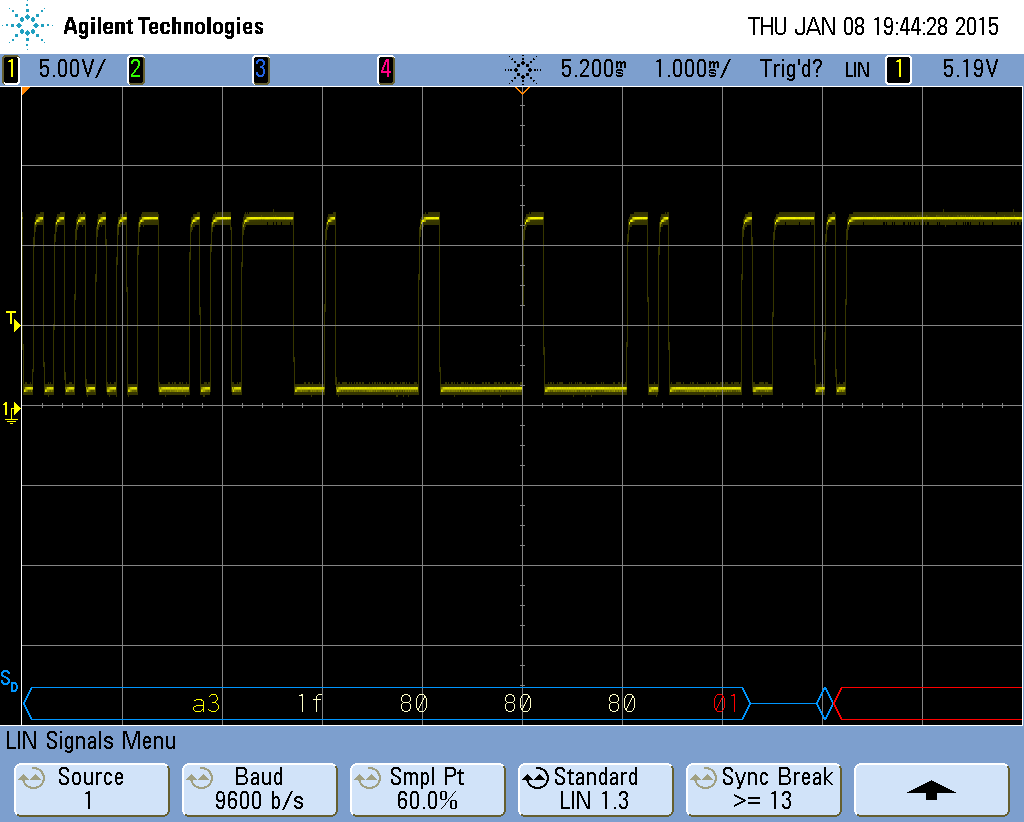
\includegraphics[width=0.9\textwidth]{releve_3.png}
\caption{Trame de commande LIN}
\end{figure}

L'analyse en champs principaux est réalisée par l'oscilloscope (en bas de l'écran). On retrouve l'identifiant et les données attendues.

\subsection{Quelle est la durée de la trame ? A quelle période minimale des signaux peuvent-ils être envoyés ? Cela correspond-il avec l'usage principal du bus LIN de transmettre des messages de commande issue d'utilisateurs ?}

La trame dure environ \SI{8}{\milli\second}, soit une période minimale de l'ordre de \SI{10}{\milli\second}. C'est amplement suffisant pour transmettre des messages issus d'utilisateurs. En effet, on peut s'attendre à ce qu'un utilisateur envoie un nouveau message au plus une fois par seconde.

\end{document}
